\section{Exercices\ldots}

	\frame
	{
		\frametitle{Pour le prochain cours}
		
		\onslide<1->
		{
			\begin{block}{Exercice 1}
				Trouver l'ensemble des attributs obligatoires pour une IRM.

				Il faudra regarder le chapitre 3 de la norme : \url{http://dicom.nema.org/standard.html}
			\end{block}
		}

		\onslide<2->
		{
			\begin{block}{Exercice 2}
				Compl\'eter le sch\'ema de la page~\ref{imageCR-IOD} :
				\begin{itemize}
					\item entit\'es ;
					\item modules ;
					\item et attributs.
				\end{itemize}
				Respectez le code couleur ou pr\'ecisez le type de module/attribut.

				Aidez-vous de la m\^eme ressource que pour l'exercice pr\'ec\'edent.
			\end{block}
		}
	}

\frame
{
	\frametitle{Exercices}
	\begin{block}{Exercice 3}
    		Trouver les erreurs dans les m\'etadonn\'ees suivantes, en fonction du tableau fourni.
    		En d\'eduire les cas qui seront rejet\'es par votre PACS.

		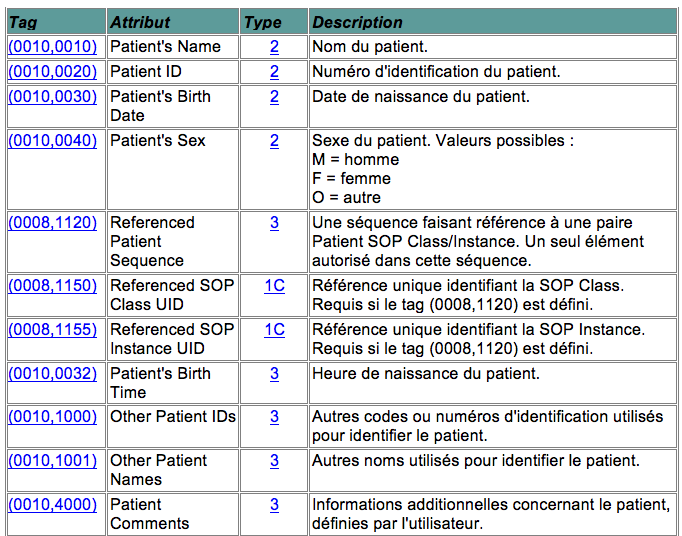
\includegraphics[width=.5\linewidth]{./figures/table.png}
		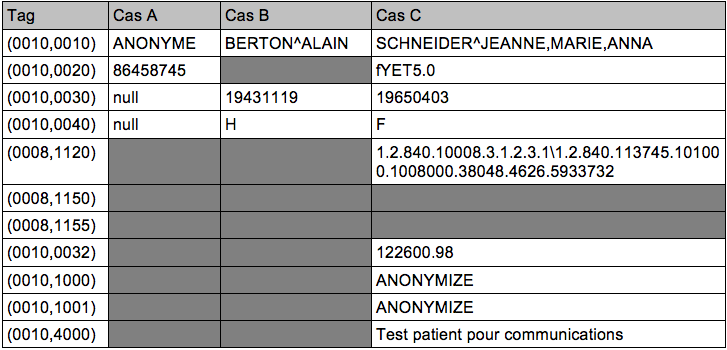
\includegraphics[width=.5\linewidth]{./figures/metadata-cases.png}
    
    		Les cases gris\'ees indiquent un champ absent, \emph{null} un champs vide.
	\end{block}
}
